\section{Introduction}
Structural restrictions can reduce uncertainty about a regression functional by more than a variance constant. Consider a four-way coefficient $B\in\R^{2\times2\times2\times2}$ whose TT rank caps are $(1,2,1)$. The outer rank-one cuts force a product of blocks of dimensions $(2,4,2)$. At $B_0=\lambda E_{0000}$, the coordinate functional $B\mapsto B_{1111}$ changes only when all three blocks change. A perturbation of Frobenius size $t$ can change this functional by order $t^3/\lambda^2$. This raises a statistical question: can an interval exploit that cubic behavior while retaining coverage over the whole rank-constrained class, including neighboring rank strata?

Existing theory makes a simple higher-order calculation insufficient as a contribution. Functional inference under degeneracy, including corrected bootstrap and minimum-distance methods, is well developed \citep{chenfang2019,bei2026}. Tensor inference with nondegenerate tangent alignment also has strong guarantees \citep{xu2025,maxia2024}. What requires a separate calculation here is the local modulus across a specified collection of TT constraints and the corresponding expected length under global honesty. In addition, structural rank restrictions may be approximate, and a small coefficient departure can be larger than a higher-order inferential scale.

We therefore study a deliberately explicit experiment: independent isotropic Gaussian designs, independent Gaussian regression errors, and a fixed-dimensional coefficient in a bounded TT rank class or a known neighborhood of that class. The main length estimand is a prespecified linear functional of the coefficient, not an individual TT core, a training-trajectory statistic, or an unobserved neural-network parameterization. Our main objective is to classify the best expected interval length at rank-one coefficients subject to coverage for every coefficient in the declared class. We allow unknown error variance but do not claim inference when ambient least squares is unavailable.

Three obstacles distinguish the calculation from a direct delta-method exercise. First, a path in an enclosing product model may violate an internal TT rank cap, so a lower modulus bound requires an actually feasible tensor path. Second, a confidence interval calibrated at the exact boundary can fail under statistically indistinguishable local changes, as Figure~\ref{fig:activation} illustrates. Third, the fitted loading projections have lower-order components even when the true ones vanish; these terms and the event of poor pilot localization must be controlled to bound expected length.

The construction uses the cuts whose rank cap equals one to partition the tensor chain. Orthogonal loading components are graded by the number of blocks perpendicular to the signal. For a fixed loading, the smallest nonzero degree determines the modulus exponent. Retaining all degrees gives a uniform formula when low-degree components approach zero. Within-block sums of two elementary products provide feasible witness paths despite the remaining TT constraints. Averaging signed paths isolates each degree without cancellation from lower ones. Confidence-ball inversion then supplies global coverage, while a graded product bound makes the calculation explicit. In the four-way example this recovers cubic inference. A six-way example with a proper singular internal rank constraint has the same cubic order, demonstrating both the scope of the classification and the limited role of that singularity.

The paper makes three claims, each proved in the appendix:
\begin{enumerate}
 \item Section~\ref{sec:theory} classifies local contact and optimal honest expected length at rank-one signals for arbitrary positive TT cap profiles, uniformly over deterministic loadings. It also shows that slack at every cut restores first-order contact for every nonzero loading.
 \item Theorem~\ref{thm:length} determines the additional length required by a known structural approximation allowance and identifies departures that cannot be detected but invalidate exact-model lengths.
 \item Section~\ref{sec:method} gives a computable, globally honest interval that attains these orders without selecting the contact order. The improved energy certificate is no longer than the original on any dataset. Section~\ref{sec:extensions} separates localization assumptions from geometry; experiments test the rate transitions, coverage distinction, and approximation sensitivity.
\end{enumerate}

\begin{figure}[t]
\centering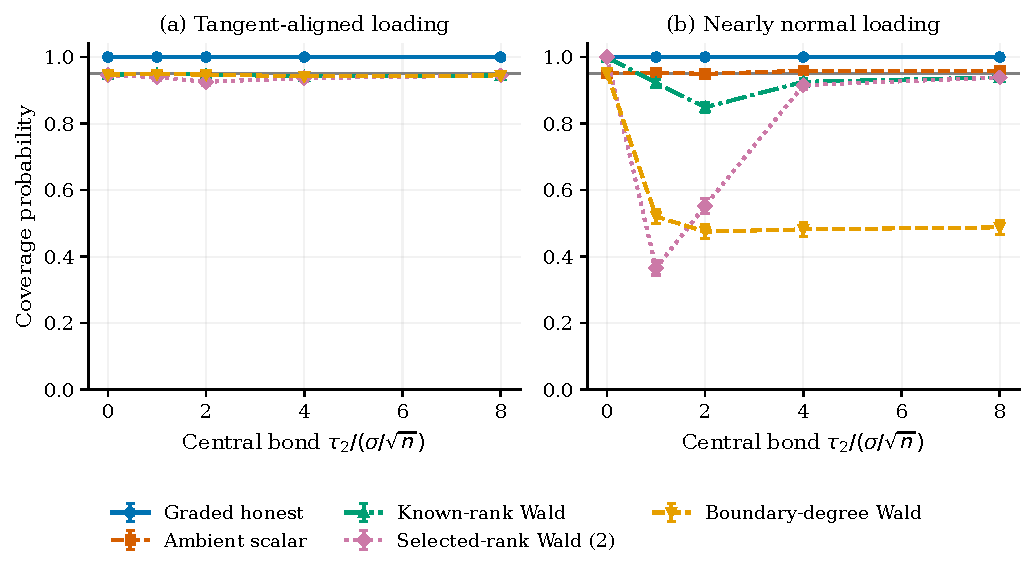
\includegraphics[width=\textwidth]{activation.pdf}
\caption{Exact-boundary calibration can fail under a local change in the central TT bond. Four binary modes have caps $(1,2,1)$, $n=2048$, $\lambda=3$, and $\sigma=0.2$; the path and two fixed loadings are specified in Section~\ref{sec:experiments}. Points use 2,000 replications with Wilson 95\% Monte Carlo intervals; the horizontal line is nominal coverage 0.95. ``Selected-rank Wald (2)'' uses the prespecified threshold multiplier two.}\label{fig:activation}
\end{figure}
